\section{Reflection security}\label{sec:refsec}

We now define the theoretical model for reflection attacks. We propose a
cryptographic game and present proofs of insecurity under the assumptions
mentioned above. We then move on to describe the necessary properties of the
various elements in the game and describe existing compression attacks,
including Rupture, as instances of the theoretical model we introduces.

\subsection{The reflection game}\label{subsec:refsecgame}

Let $\mathcal{SE} = (Gen, \mathcal{E}, \mathcal{D})$ be a private-key encryption
scheme, $\mathcal{A}$ be an adversary and $\mathcal{S}$ be a simulator of
$\mathcal{A}$. Also let a rendering function $f(\cdot, \cdot)$, some function
$g$ of a plaintext, and a distribution of secrets $\mathcal{M}$. We require that
the rendering function $f$ is polynomially computable and reversible. The game
$\text{Game}_{\text{REF-SEC}}^{\mathcal{SE},\mathcal{A}}(\lambda)$ is
parameterized with the security parameter $\lambda$.

In the case of the example described above, the rendering function $f$ is the
rendering of the HTML response along with compression that is applied on it.
Function $g$ represents the prefix of the secret $s$ in the plaintext response.

The challenger produces a $\lambda$-bit key $k \leftarrow Gen(1^\lambda)$. The
challenger initially chooses a secret $s \leftarrow \mathcal{M}$.

The adversary is then allowed to run and make arbitrary calls to a reflection
oracle. The oracle is parameterized by $s$, the secret unknown to the adversary.
For the reflection oracle call, the adversary chooses a reflection string $r$
and sends it to the oracle. The oracle computes $m = f(s, r)$. Subsequently $m$
is encrypted as $c = \mathcal{E}_\kappa(m)$, and $c$ is sent back to the
adversary.

When the adversary decides to complete the game, they output a guess $y$. The
adversary is successful if $g(s) = y$. In the case of Rupture, a successful
attack results in the decryption of a single character that extends the known
prefix of secret $s$.

Formally, let the public key adversarial game be defined as follows:

\begin{lstlisting}[texcl,mathescape,basicstyle=\small]
def $\text{Game}_{\text{REF-SEC}}^{\mathcal{SE},\mathcal{A}}(\lambda)$:
    $k \leftarrow Gen(1^\lambda)$
    $s \leftarrow \mathcal{M}$
    $y \leftarrow \mathcal{A}^{\text{Reflect}^{k}_s(r)}(1^\lambda)$
    if $y = g(s)$:
        return 1
    else:
        return 0
\end{lstlisting}

Where the reflection oracle provided to the adversary is as follows:

\begin{lstlisting}[texcl,mathescape,basicstyle=\small]
def $\text{Reflect}^{k}_s(r)$:
    $m = f(s, r)$
    $c \leftarrow \mathcal{E}_{k}(m)$
    return $c$
\end{lstlisting}

Let the simulator game be defined as follows:

\begin{lstlisting}[texcl,mathescape,basicstyle=\small]
def $\text{Game}_{\text{REF-SIM}}^{\mathcal{SE},\mathcal{S}}(\lambda)$:
    $y \leftarrow \mathcal{S}(1^\lambda)$
    $s \leftarrow \mathcal{M}$
    if $y = g(s)$:
        return 1
    else:
        return 0
\end{lstlisting}

Where the simulator does not require an oracle for its execution.

The reflection game is depicted in Figure \ref{fig:refgame}.

    \begin{figure}[thpb]
        \centering
            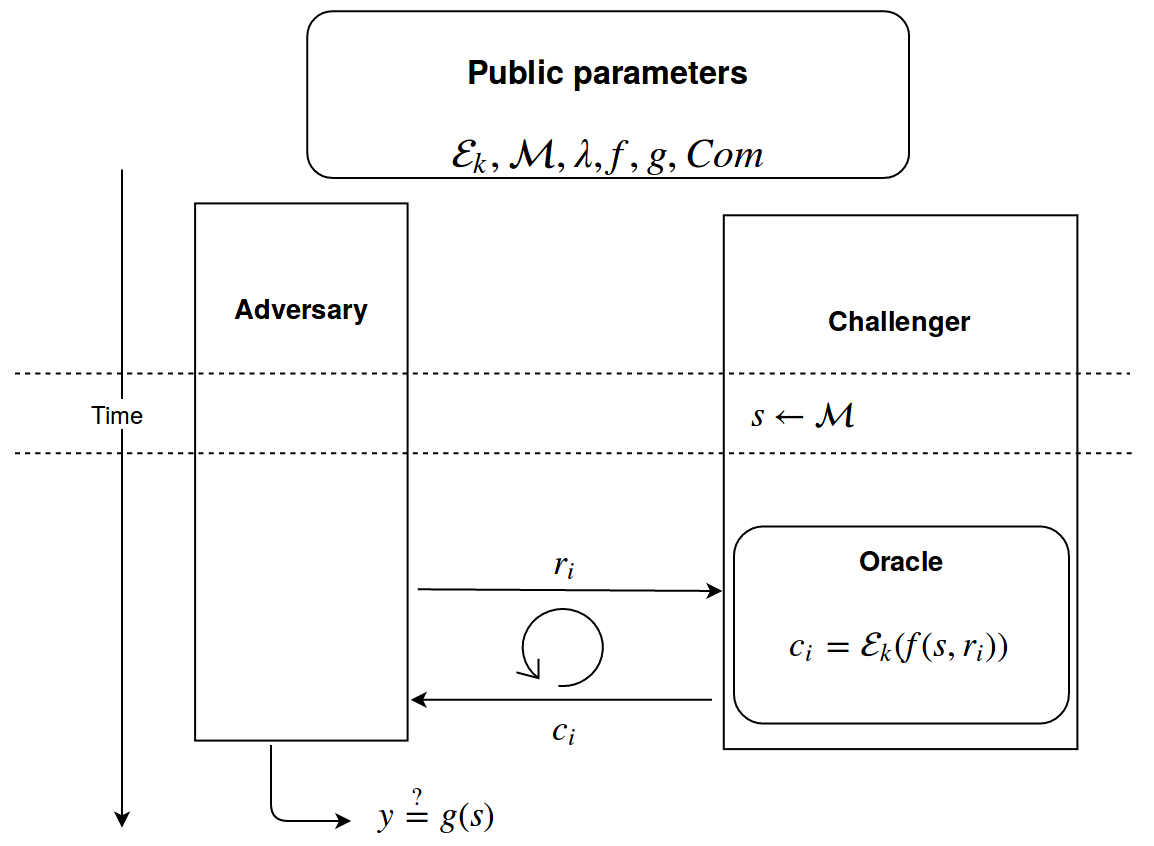
\includegraphics[width=0.48\textwidth]{figures/reflection_game.png}
        \caption{Reflection Game}
        \label{fig:refgame}
    \end{figure}

\subsection{Adversarial advantage}\label{subsec:refsecadv}

Let us now define the advantage of the adversary against a simulator:
\begin{align*}
    \text{Adv}_{\mathcal{SE}, \mathcal{A}, \mathcal{S}}&(\lambda) &\defeq\\
    |\Pr[\text{Game}_{\text{REF-SEC}}^{\mathcal{SE},\mathcal{A}}(\lambda) = 1] &-\\
    \Pr[\text{Game}_{\text{REF-SIM}}^{\mathcal{SE},\mathcal{S}}(\lambda) = 1]| &
\end{align*}

\subsection{Adaptive reflection security}\label{subsec:adaptiverefsec}

Given a rendering function $f(\cdot, \cdot)$, a public-key encryption
scheme $\mathcal{SE}$ is \textit{reflection-secure} if:
\begin{align*}
    \forall \mathcal{M}:
    \forall g:
    \forall PPT \mathcal{A}:
    \exists PPT \mathcal{S}:\\
    \text{Adv}_{\mathcal{SE}, \mathcal{A}, \mathcal{S}}(\lambda) = negl(\lambda)
\end{align*}

\begin{lemma}[Semantic security]
    Let $(Gen, K, D)$ be a length-preserving reflection-secure encryption
    scheme. Then it is also semantically secure.
\end{lemma}

For a full proof, see Appendix A.
